\chapter{Introducción a Python}
\section{Nociones básicas}
\emph{Python} es un lenguaje de programación interpretado de alto nivel cuyas características permiten su uso en diversas disciplinas. Los lenguajes de alto nivel en programación poseen una sintaxis que se asemeja al lenguaje humano, lo que facilita la claridad y legibilidad del código, haciendo su escritura y comprensión más accesibles. En contraste, los lenguajes de bajo nivel, como el \emph{ensamblador}, utilizan una sintaxis más cercana al lenguaje máquina, lo que los hace más eficientes para la computadora pero más complejos de leer y escribir para los humanos.

Python, al ser un lenguaje interpretado, traduce y ejecuta el código línea por línea durante la ejecución, lo que puede resultar en tiempos de ejecución más largos en comparación con los lenguajes compilados, que se traducen en código máquina antes de ejecutarse. Sin embargo, esta diferencia en el tiempo de ejecución suele ser insignificante en muchos casos prácticos. Además, el tiempo requerido para desarrollar y mantener código en Python es considerablemente menor comparado con los lenguajes de bajo nivel, equilibrando así el tiempo total de desarrollo.

Adicionalmente, Python permite la integración de bibliotecas y códigos escritos en otros lenguajes de programación, aprovechando sus ventajas y capacidades para mejorar el rendimiento. Esta flexibilidad y facilidad de uso han contribuido a que Python se convierta en uno de los lenguajes de programación más populares en la actualidad, especialmente en los campos de ciencias e ingeniería.

En esta primera clase revisaremos algunos conceptos básicos de Python, cómo instalarlo en cualquier sistema operativo y además elegiremos un entorno de desarrollo integrado para escribir nuestros códigos Python. 

\section{Python en diferentes sistemas operativos}
Python es un lenguaje de programación multiplataforma, esto significa que puede utilizarse en todos los sistemas operativos principales. Sin embargo, los métodos de instalación difieren dependiendo de cada sistema operativo. El objetivo de esta sección es que puedas ejecutar el famoso programa <<¡Hola Mundo!>> usando Python en tu sistema operativo. Ten en cuenta que trabajaremos exclusivamente con Python 3.

\subsection{Python en Windows}
Por lo general, Windows no cuenta con una versión de Python por defecto, por lo que será necesario instalarlo además de un editor de texto. Para verificar si tu versión de Windows cuenta con Python, primero debes abrir el menú de inicio, escribir los caracteres \mintbold{bash}{cmd} y hacer clic sobre la aplicación llamada \emph{símbolo del sistema}. Esto abrirá una terminal de comandos en la que deberás escribir las palabras \mintbold{bash}{python --version} (todo en minúsculas) y presiona la tecla Enter. 

Si el resultado es algo similar a \mintbold{bash}{3.x.x}, entonces Python ya está instalado en tu sistema. Sin embargo, si el resultado es un mensaje que dice que \mintinline{bash}{python} no es un comando reconocido, entonces sigue las siguientes instrucciones para instalarlo.

\begin{enumerate}
    \item \textbf{Descarga el instalador de Python.} Abre tu navegador y dirígete a la página \url{https://www.python.org/downloads/}. Haz clic en el botón que dice <<Download Python 3.x.x>> (donde <<3.x.x>> es la versión más reciente). 
    
    \item \textbf{Ejecuta el instalador.} Encuentra el archivo del instalador que acabas de descargar (normalmente estará en tu carpeta de descargas) y haz doble clic para ejecutarlo.
    En la primera ventana del instalador, asegúrate de marcar la casilla que dice <<Add Python 3.x to PATH>>. Esto es importante para que puedas usar Python desde terminal de comandos sin problemas. Finalmente, haz clic en <<Install Now>> para comenzar la instalación.
    
    \item \textbf{Verifica la instalación.} Una vez que finalice la instalación, abre una nueva terminal de comandos y escribe las palabras \mintbold{bash}{python --version}. Esto debería mostrar la versión de Python que has instalado.
\end{enumerate}

\subsection{Python en Linux}
Cualquier sistema operativo Linux cuenta con una versión de Python instalada por defecto. Por lo tanto, solo necesitas verificar cuál versión tienes instalada en tu sistema. Para lograrlo, abre una terminal de comandos con la combinación de teclas \mintinline{bash}{Ctrl+Alt+T} y escribe las palabras \mintbold{bash}{python --version} (todo en minúsculas) y presiona la tecla Enter. Si el resultado es un mensaje similar a \mintbold{bash}{2.x.x} o si en cambio te aparece un mensaje que dice que el comando \mintinline{bash}{python} no fue encontrado, entonces intenta escribiendo \mintbold{bash}{python3 --version} y presiona Enter. El resultado debería ser algo como \mintbold{bash}{3.x.x}.

\subsection{Python en Mac OSX}
La mayoría de los sistemas Mac OSX cuenta con al menos una versión de Python instalada por defecto. Esto significa que es posible que cuentes con dos versiones, para verificarlo, abre una terminal de comandos haciendo clic en \mintbold{bash}{Aplicaciones > Utilidades > Terminal}. Ahora escribe las palabras \mintbold{bash}{python --version} (todo en minúsculas) y presiona la tecla Enter. 

Al igual que con los sistemas Linux, es posible que el resultado sea un error o un mensaje con algo similar a \mintbold{bash}{2.x.x}, lo que significa que la versión instalada es Python 2. Si cualquiera de las dos opciones anteriores es cierta, intenta escribiendo en la terminal \mintbold{bash}{python3 --version} y presiona Enter. Si el resultado es algo similar a \mintbold{bash}{3.x.x}, entonces cuentas con una versión de Python 3.

Si por algún motivo al escribir \mintbold{bash}{python3 --version} obtienes un error, entonces necesitas instalar Python 3 en tu sistema. Para eso, sigue los siguientes pasos.

\begin{enumerate}
    \item \textbf{Descarga el instalador.} Dirígete a la página \url{https://www.python.org/}. Coloca el cursor sobre el botón <<Downloads>> y selecciona <<macOS>>. En la página de descargas deberías ver un botón llamado \mintbold{bash}{macOS 64-bit universal2 installer} debajo del título <<Stable Releases>>. Haz clic sobre ese botón para descargar el instalador con extensión \mintbold{bash}{.pkg}

    \item \textbf{Ejecuta el instalador.} Una vez que el archivo \mintbold{bash}{pkg} se haya descargado, haz doble clic en él para iniciar el proceso de instalación. Aparecerá una ventana del asistente de instalación. Sigue las instrucciones en pantalla. Generalmente, solo necesitas hacer clic en <<Continuar>> y luego en <<Instalar>>. El instalador pedirá tu contraseña de administrador para proceder. Una vez que se complete el proceso, haz clic en <<Cerrar>> para terminar.

    \item \textbf{Verifica la instalación.} Abre una nueva terminal de comandos y escribe las palabras \mintbold{bash}{python3 --version}. El resultado debería ser la versión de Python que acabas de instalar.
\end{enumerate}

\section{Ejecutando Python}
Para comenzar a usar Python, solo tienes que abrir una terminal de comandos, escribir la palabra \mintbold{bash}{python3} y presionar la tecla Enter (Nota: este documento fue escrito en un sistema Linux, si en cambio estás usando Windows, para ejecutar Python solo debes escribir \mintbold{bash}{python} en la terminal de comandos, sin agregar el número \mintbold{bash}{3}. Ten esto en cuenta en todo el documento a partir de este momento). El resultado debe ser algo similar a lo siguiente:

\begin{terminal}[Terminal]
Python 3.10.12 (main, Jul 29 2024, 16:56:48) [GCC 11.4.0] on linux
Type "help", "copyright", "credits" or "license" for more information.
>>> 
\end{terminal}
Este mensaje nos muestra información sobre la versión de Python instalada, el sistema operativo en el que se instaló e información general. Inmediatamente después, aparece una línea con el símbolo \mintbold{bash}{>>>}, el cual es conocido como el <<Intérprete de Python>> (en inglés: \emph{Python prompt}). El intérprete de Python nos indica que podemos ingresar nuestros comandos desde ahí y serán ejecutados al presionar la tecla Enter.

Para nuestro primer ejemplo usaremos la función \mintinline{python}{print} definida por defecto en Python. Escribe el comando \mintinline{python}{print("¡Hola mundo!")} en tu sesión de Python y presionamos Enter. El resultado debería ser el siguiente:

\begin{terminal}[Terminal]
>>> print("¡Hola mundo!")
¡Hola mundo!
>>> 
\end{terminal}

Como puedes ver, la instrucción que se utilizó para mostrar el mensaje <<¡Hola mundo!>> es muy similar al lenguaje humano. Además, en la línea siguiente aparece de nuevo el intérprete de Python. Esto nos indica que Python está listo para seguir recibiendo instrucciones.

Para salir de Python y volver a una terminal de comandos normal, debes utilizar la función \mintinline{pycon}{exit} también definida por defecto. Específicamente, debes escribir el comando \mintinline{python}{exit()} y presionar Enter.

Esta es la forma más simple de ejecutar comandos de Python. Afortunadamente, no es la única. Para los propósitos del curso, necesitaremos de un Entorno de Desarrollo Integrado (IDE, por sus siglas en inglés). 

\subsection{Creando un entorno virtual}
Antes de continuar e independientemente de tu sistema operativo, es conveniente crear un entorno virtual de Python para evitar cualquier problema de compatibilidad con el sistema operativo y que las cosas funcionen correctamente. Primero debes abrir una nueva terminal de comandos e instalar el paquete \mintinline{bash}{virtualenv}, ejecutando la instrucción:

\begin{shell}
pip install virtualenv
\end{shell}

 Cuando termine, escribe la siguiente instrucción para crear un entorno virtual llamado <<\mintinline{bash}{omm}>> (puedes cambiar la palabra \mintinline{bash}{omm} a cualquier otro nombre que prefieras, pero debe ser una única palabra, sin espacios):

\begin{shell}
python3 -m venv omm
\end{shell}

El comando anterior creó un directorio llamado <<\mintinline{bash}{omm}>> (o el nombre que hayas elegido) en el directorio en el que abriste la terminal de comandos. Por defecto, la terminal de comandos se abre en el directorio <<\mintinline{shell-session}{C:\Users\user}>> en Windows, y en el directorio <<\mintinline{bash}{/home/user/}>> en Linux/MacOSX (donde \mintinline{bash}{user} es tu nombre de usuario en tu computadora, independientemente de tu sistema operativo). 

Para activar el entorno virtual en Windows, debes ejecutar el siguiente comando:
\begin{shell}
C:\Users\user\omm\Scripts\activate 
\end{shell}
Ten en cuenta que debes cambiar la palabra \mintinline{bash}{user} por tu nombre de usuario.

En cambio, para activarlo en Linux y Mac OSX, se hace con el comando:
\begin{shell}
source ~/omm/bin/activate
\end{shell}

Como resultado, verás que a la izquierda de tu terminal de comandos aparece el nombre de tu entorno virtual encerrado en paréntesis, esto indica que está activado. Deberás ejecutar este comando para utilizar el entorno virtual de Python cada vez que abras una nueva terminal. Para desactivarlo, debes escribir el comando \mintbold{bash}{deactivate} y ejecutarlo.

\subsection{El editor Geany}
Un programa de Python es simplemente un archivo de texto con extensión \mintinline{bash}{.py} que puede escribirse en cualquier editor de texto. 
Existen muchos editores de texto y puedes usar el que prefieras. Recomiendo usar Geany porque es bastante simple, es ligero y fácil de instalar. Además permite ejecutar los programas directamente desde el editor, también utiliza el resaltado de sintaxis y permite usar una terminal integrada para ejecutar los códigos si así lo prefieres. 

\subsubsection{Geany en Windows}
Para instalar Geany en Windows, dirígete a la página \url{https://www.geany.org/download/releases/} y descarga el instalador para Windows. Una vez que se haya descargado el archivo \mintinline{bash}{.exe}, haz doble clic en él para iniciar el proceso de instalación. Sigue las instrucciones del asistente de instalación. Puedes dejar las opciones predeterminadas, a menos que desees personalizar la instalación.


 \subsubsection{Configuración de Geany en Windows}
Una vez instalado, abre Geany desde el menú de aplicaciones. En la ventana del editor, escribe la instrucción \mintbold{python}{print("¡Hola mundo!")} y utiliza la combinación de teclas \mintbold{bash}{Ctrl+S} para guardar el archivo. Puedes guardar el archivo con el nombre \mintinline{bash}{hello_world.py} en tu carpeta de trabajo. Asegúrate de colocar la extensión \mintinline{bash}{.py} en el nombre de tu archivo al momento de guardarlo. 

Para que Geany funcione correctamente con el entorno virtual, se debe hacer una configuración sencilla. Dentro de la ventana de Geany, dirígete a \mintinline{bash}{Build -> Set Build Commands}. Ahora haz lo siguiente:
\begin{enumerate}
    \item En el campo llamado <<\mintinline{bash}{Compile}>>, edita su contenido para que el comando tenga lo siguiente: \mintinline{shell-session}{C:\Users\user\omm\Scripts\python -m py_compile "%f"} 

    \item En el campo llamado <<\mintinline{bash}{Execute}>>, edita su contenido para que el comando tenga lo siguiente: \mintinline{shell-session}{C:\Users\user\omm\Scripts\python "%f"} 

    \item Haz clic en OK para guardar los cambios.
\end{enumerate}

Usa las opciones de \mintinline{bash}{Build} o los atajos de teclado (por ejemplo, \mintinline{bash}{F8} para compilar y \mintinline{bash}{F5} para ejecutar) para compilar y ejecutar el archivo Python. Verifica que el intérprete de Python utilizado sea el del entorno virtual y no el global.

El resultado debería ser un mensaje que dice <<¡Hola mundo!>>, tal como cuando se ejecutó el comando desde una terminal.

\subsubsection{Geany en Linux y Mac OSX}
Para instalar Geany en Linux, es suficiente con que ejecutes los siguientes comandos en una terminal:
\begin{shell}[Instalar Geany en Linux]
sudo apt update
sudo apt install geany
\end{shell}

En Mac OSX, puedes usar \mintinline{bash}{Homebrew} para instalar Geany desde una terminal con el comando:

\begin{shell}[Instalar Geany en Mac OSX]
brew install --cask geany
\end{shell}

La configuración de Geany en Linux y Mac OSX es la misma. Para hacerlo, sigue los pasos descritos en la sección <<Configuración de Geany en Windows>> con la única diferencia que el campo <<\mintinline{bash}{Compile}>> debe contener lo siguiente: \mintinline{shell-session}{/home/user/omm/bin/python -m py_compile "%f"}  y el campo <<\mintinline{bash}{Execute}>> debe tener: \mintinline{shell-session}{/home/user/omm/bin/python "%f"}.

Ten en cuenta que tanto en Windows como en Linux y Mac OSX, debes reemplazar la palabra <<\mintinline{bash}{user}>> por tu nombre de usuario. Utilizaremos Geany principalmente para escribir y editar algunas funciones que utilizaremos. Ahora revisaremos algunos IDEs un poco más avanzados y que permiten hacer más cosas.

\subsection{Jupyter Notebook}
Jupyter Notebook es un IDE de Python basado en navegadores web, que además de ejecutar códigos de Python, permite incluir texto con formato, ecuaciones, imágenes y mucho más. Esencialmente, es un cuaderno donde es posible escribir código y tomar apuntes. Para instalarlo debes abrir una nueva terminal, activar el entorno virtual que creaste anteriormente y ejecutar la instrucción \mintbold{bash}{pip install notebook}. En una terminal se vería así:

\begin{shell}
source ~/omm/bin/activate
pip install notebook
\end{shell}
Recuerda utilizar los comandos adecuados si usas Windows. Una vez que termine la instalación, puedes usar Jupyter Notebook escribiendo la instrucción \mintbold{bash}{jupyter notebook} (separado y en minúsculas) en la misma terminal de comandos. Esto abrirá una nueva pestaña en tu navegador predeterminado y te mostrará un explorador de archivos con el contenido de la carpeta donde ejecutaste la instrucción anterior, como se muestra en la Figura \ref{fig:jupyter-interface}

\begin{figure}[htb]
    \centering
    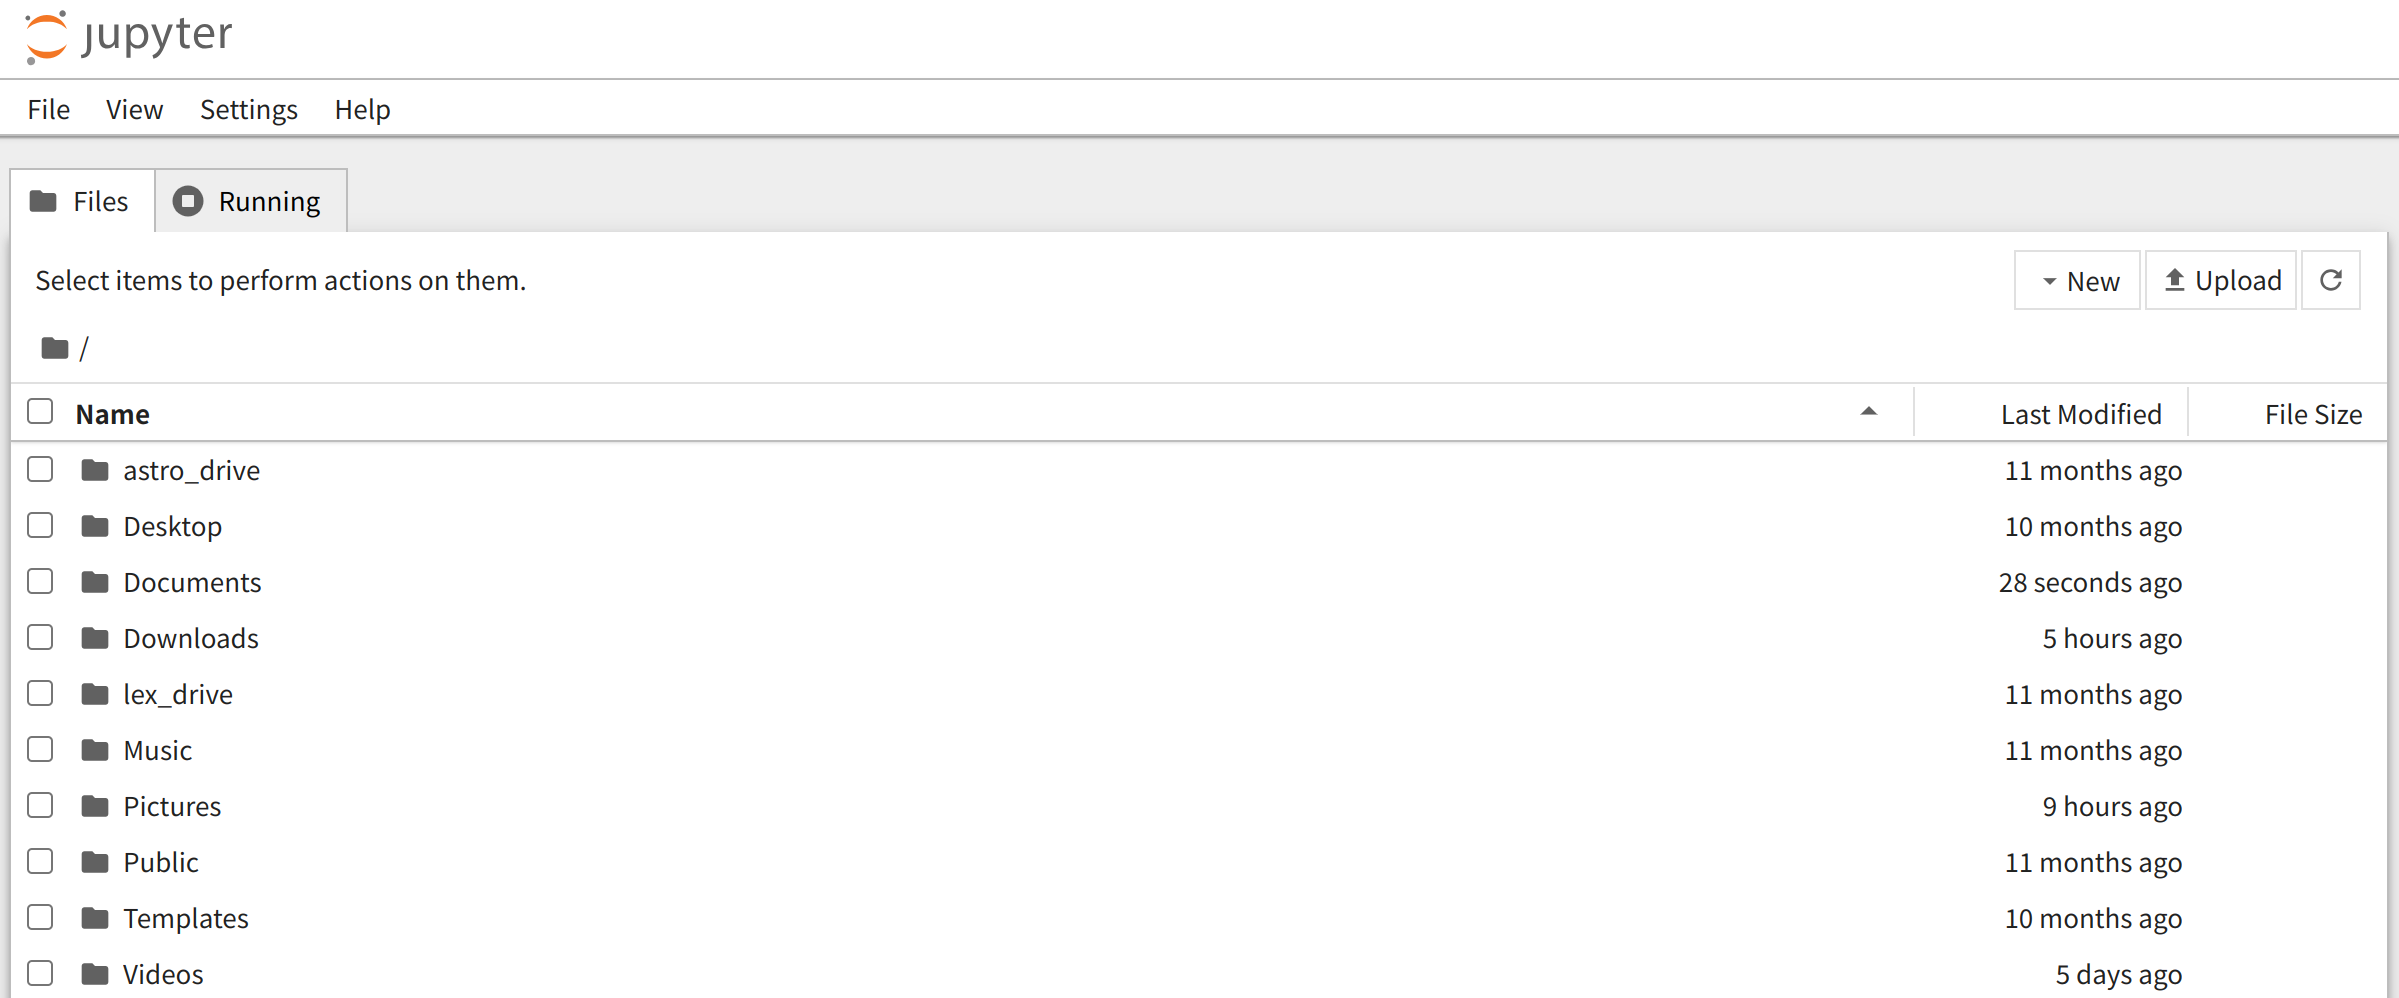
\includegraphics[width=\linewidth]{figures/jupyter-interface.png}
    \caption{Interfaz gráfica de Jupyter Notebook}
    \label{fig:jupyter-interface}
\end{figure}

Desde la interfaz de Jupyter dirígete a tu carpeta de trabajo y crea un nuevo Notebook. Para lograrlo, haz click en el botón <<\mintinline{bash}{New}>> en la esquina superior derecha y selecciona la opción <<\mintinline{bash}{Notebook}>>, luego elige el \emph{kernel} llamado <<\mintinline{bash}{Python 3 (ipykernel)}>> y esto abrirá una nueva pestaña en tu navegador. 

\begin{figure}[htb]
    \centering
    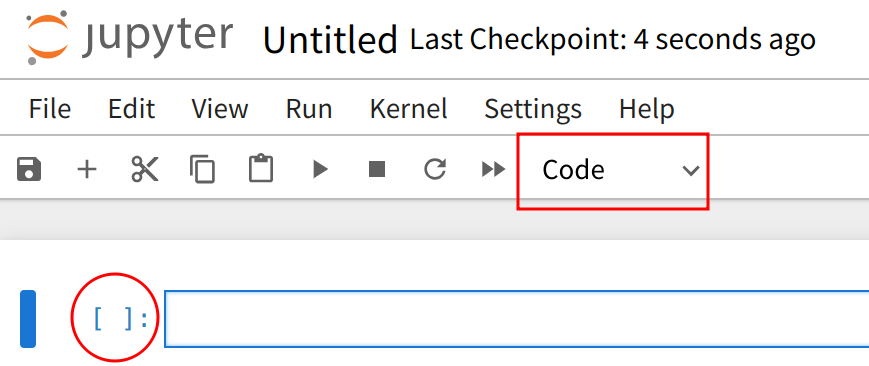
\includegraphics[width=0.48\linewidth]{figures/Jupyter-code.png} \hfill 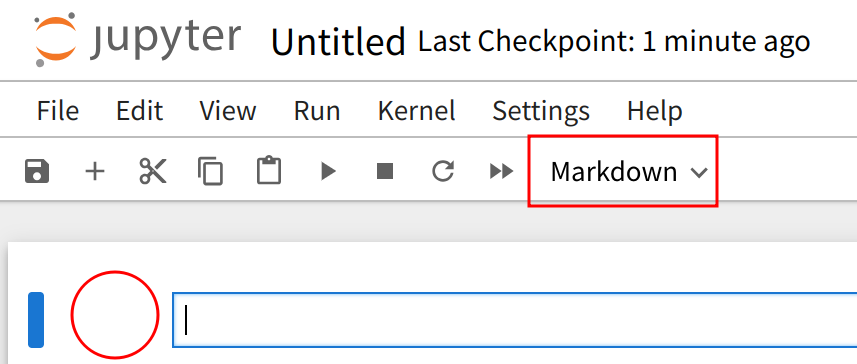
\includegraphics[width=0.48\linewidth]{figures/jupyter-markdown.png}
    \caption{Opciones disponibles para escribir en Jupyter}
    \label{fig:jupyter-code-markdown}
\end{figure}

En esa nueva pestaña, verás que aparecen los caracteres \mintinline{python}{[]:} (encerrado con un círculo rojo en el panel izquierdo de la Figura \ref{fig:jupyter-code-markdown}) y a la derecha aparece una celda vacía donde puedes escribir los comandos de Python. Los caracteres \mintinline{python}{[]:} en Jupyter Notebook son el equivalente a los caracteres \mintbold{python}{>>>} en la terminal. 

En la parte superior del Notebook hay una barra de menú, que a su vez contiene un botón con la palabra <<\mintinline{bash}{Code}>> (encerrada con un rectángulo rojo en el panel izquierdo de la Figura \ref{fig:jupyter-code-markdown}). Al darle clic se muestra un menú desplegable cuyas opciones son <<\mintinline{bash}{Code}>> y <<\mintinline{bash}{Markdown}>>. Este último es un tipo de \emph{lenguaje de marcas} bastante popular para escribir texto con formato. Si seleccionas <<\mintinline{bash}{Markdown}>>, los símbolos \mintinline{python}{[]:} de la celda desaparecen (como se muestra en el panel derecho de la Figura \ref{fig:jupyter-code-markdown}) y ahora puedes escribir texto, ecuaciones, imágenes y más. Puedes revisar algunas nociones básicas sobre la escritura de texto Markdown en este enlace de \href{https://docs.github.com/en/get-started/writing-on-github/getting-started-with-writing-and-formatting-on-github/basic-writing-and-formatting-syntax}{Github Docs}. 

Cuando vas a escribir código, siempre debes verificar que la celda está en modo <<\mintinline{bash}{Code}>> o en su defecto, que a la izquierda de la celda aparezcan los símbolos \mintinline{python}{[]:}, de lo contrario, tus comandos no se ejecutarán. Por ejemplo, da clic en la celda vacía y asegúrate que se encuentre en modo <<\mintinline{bash}{Code}>> y escribe el comando \mintbold{python}{print("¡Hola mundo!")}. Para ejecutar el código de una celda, debes dar click a la celda y usar la combinación de teclas \mintbold{bash}{Shift+Enter}. El resultado debería ser algo similar a lo siguiente:

\begin{pyin}
print("¡Hola mundo!")
\end{pyin}
\begin{pyprint}
¡Hola mundo!
\end{pyprint}

Para cerrar correctamente Jupyter Notebook, dirige tu cursor hacia la esquina superior izquierda del Notebook y selecciona \mintinline{bash}{File -> Shutdown}. Una vez que lo hagas, podrás cerrar esa pestaña del navegador. Debes repetir este procedimiento para todas las pestañas del Notebook abiertas. Como último dato sobre Jupyter Notebook, debes saber que aunque necesite de un navegador web para funcionar, en realidad no necesita de una conexión a internet para ejecutar los comandos. El navegador web es únicamente para la interfaz gráfica.

\subsection{Visual Studio Code y PyCharm}
Visual Studio Code (VS Code) y PyCharm son otros IDEs muy populares que también trabajan con Notebooks de Python y también archivos de texto plano con extensión \texttt{.py}. Su interfaz es similar a la de Jupyter Notebook y funcionan de la misma manera. Puedes revisar las instrucciones de instalación y configuración de VS Code y PyCharm en los sitios web oficiales \url{https://code.visualstudio.com/} y \url{https://www.jetbrains.com/es-es/pycharm/download/}, respectivamente. 

Como última opción, si no te es posible instalar Python en tu computadora, puedes utilizar la opción en línea llamada Google Colaboratory (o simplemente Colab), a la que puedes acceder desde tu cuenta de google drive. La ventaja de usar Colab es que no necesitas instalar nada en tu computadora y puedes usar todos los paquetes de Python que requieras. Sin embargo, sí necesitarás de una conexión a internet para poder utilizarlo.

PyCharm, VS Code, Colab y Jupyter Notebook son totalmente equivalentes entre sí, teniendo diferencias mínimas y por lo tanto puedes utilizar el IDE que sea de tu preferencia. Teniendo esto en cuenta, podemos iniciar con algunas nociones sobre la escritura de código Python usando Notebooks.

\section{Python como calculadora}
\subsection{Operaciones aritméticas}
Una de las formas elementales en las que Python puede ser utilizado es como una calculadora. En este sentido, la Tabla \ref{tab:aritmetic-operators} muestra las operaciones aritméticas que pueden ejecutarse con Python. Quizá no estés muy familiarizado con las operaciones de división entera (representada con los caracteres \mintinline{python}{//}) y división modular (representada con el carácter \mintinline{python}{%}), pero las revisaremos con detalle más adelante.

\begin{table}[htb]
    \centering
    \caption{Operadores aritméticos}
    \label{tab:aritmetic-operators}
    \begin{tabular}{c|c} \hline
        Símbolo/Operador & Significado/Operación \\ \hline
        + & Suma \\
        - & Resta \\
        * & Multiplicación \\
        / & División \\
        ** & Exponenciación \\
        // & División entera \\
        \% & División modular \\ \hline
    \end{tabular} 
\end{table}

Abre una nueva terminal de comandos, activa tu entorno virtual de Python e inicia una nueva sesión de Jupyter Notebook. Puedes abrir el mismo Notebook que creaste anteriormente o crear uno nuevo. Asegúrate que las celdas estén en modo <<\mintinline{bash}{Code}>> e intenta ejecutar los siguientes comandos. El resultado de cada comando se mostrará al lado de los caracteres {\color{myorange}\mintinline{python}{[]:}} (en color naranja). 

Veamos cómo funcionan los operadores aritméticos con unos ejemplos sencillos. Comenzamos con una simple, para calcular el valor de la operación $5+9$:

\begin{pyin}
5 + 9
\end{pyin}
\begin{pyout}
14
\end{pyout}

La siguiente expresión es equivalente a $40 - 5\times 4$:
\begin{pyin}
40 - 5*4
\end{pyin}
\begin{pyout}
20
\end{pyout}

Y también podemos agrupar términos utilizando los paréntesis. Por ejemplo, podemos calcular el valor de la expresión $(40 - 5\times 4)/4$ usando la siguiente sintaxis:
\begin{pyin}
(40 - 5 * 4) / 4
\end{pyin}
\begin{pyout}
5.0
\end{pyout}

Y para calcular el valor de $3^2 + 4^2$ se usa la sintaxis:
\begin{pyin}
4**2 + 3**2
\end{pyin}
\begin{pyout}
25
\end{pyout}

Ahora revisemos con un poco de detalle el operador \mintinline{python}{//}, que en Python es el operador de división entera. Este operador divide dos números y redondea el resultado hacia abajo al número entero más cercano. Por ejemplo, sabemos que $7/3 = 2.333$. Si aplicamos el operador de división entera a esos mismos números se obtiene:
\begin{pyin}
7 // 3
\end{pyin}
\begin{pyout}
2
\end{pyout}

En este caso, \mintinline{python}{7 // 3} es igual a $2$ porque la parte fraccionaria ($0.333...$) se descarta. Ahora veamos cómo se comporta este operador con números negativos:
\begin{pyin}
-7 // 3
\end{pyin}
\begin{pyout}
-3
\end{pyout}

En este caso, \mintinline{python}{-7 // 3} es igual a \mintinline{python}{-3} porque el resultado se redondea hacia abajo (es decir, al entero más negativo).

Por otro lado, el operador \% en Python es el operador de división modular (también conocido como resto o residuo). Este operador devuelve el resto de la división entre dos números. Es útil para determinar si un número es divisible por otro, o para obtener la parte sobrante después de dividir un número por otro. Veamos cómo funciona con ejemplos:
\begin{pyin}
7 % 3
\end{pyin}
\begin{pyout}
1
\end{pyout}
En este caso, \mintinline{python}{7 % 3} es igual a $1$ porque $7$ dividido entre $3$ es igual a $2$ con un residuo de $1$.

\subsection{Operaciones matemáticas avanzadas}
Para realizar operaciones matemáticas más avanzadas, necesitaremos utilizar un \emph{módulo} de Pytho llamado \mintinline{python}{math}. Un módulo es un archivo que contiene definiciones y declaraciones de Python, como funciones, variables y clases. Los módulos permiten organizar y reutilizar código.

Para usar el módulo \mintinline{python}{math}, debemos importarlo en nuestro código. La forma más sencilla de hacerlo es usando la palabra clave <<\mintinline{python}{import}>>. Dentro del módulo \mintinline{python}{math} están definidas muchas funciones matemáticas como la raíz cuadrada, logaritmos, funciones trigonométricas y mucho más. Para usarlas, debemos hacerlo con el operador de acceso, que en Python es un punto. La siguiente celda de código muestra cómo importar el módulo \mintinline{python}{math} y cómo acceder a la función raíz cuadrada, definida como \mintinline{python}{sqrt} dentro de dicho módulo:

\begin{pyin}
import math

print(math.sqrt(16))
\end{pyin}
\begin{pyprint}
4.0
\end{pyprint}

También podemos hacer importaciones específicas de las funciones dentro del módulo. Para esto usamos la palabra <<\mintinline{python}{from}>>. El siguiente ejemplo muestra cómo importar la función \mintinline{python}{sqrt} definida dentro del módulo \mintinline{python}{math}:
\begin{pyin}
from math import sqrt

print(sqrt(16))
\end{pyin}
\begin{pyprint}
4.0
\end{pyprint}
En este último caso, no fue necesario escribir \mintinline{python}{math.sqrt} para calcular la raíz cuadrada, porque importamos directamente la función \mintinline{python}{sqrt}. 

Adicionalmente, puedes importar módulos o funciones específicas y renombrarlas a tu gusto usando la palabra <<\mintinline{python}{as}>>. Los siguientes dos ejemplos muestran cómo funciona esta sintaxis.

\begin{pyin}
import math as m

print(m.sqrt(16))
\end{pyin}
\begin{pyprint}
4.0
\end{pyprint}

\begin{pyin}
from math import sqrt as raiz_cuadrada

print(raiz_cuadrada(16))
\end{pyin}
\begin{pyprint}
4.0
\end{pyprint}

Como normal general, se recomienda hacer todas las importaciones al inicio del programa y utilizar alias claros y fácilmente identificables. 
